\documentclass[11pt]{article}
\usepackage[a4paper,margin=1in]{geometry}
\usepackage{amsmath,amssymb,booktabs,array,graphicx,float}
\usepackage[T1]{fontenc}
\usepackage{lmodern}
\usepackage{microtype}
\usepackage{hyperref}
\usepackage{enumitem}
\usepackage{tikz}
\usetikzlibrary{arrows.meta,positioning,fit,calc}
\usepackage[most]{tcolorbox}
\graphicspath{{e2c_explained_figs/}}
\setlength{\parskip}{0.5em}
\setlength{\parindent}{0pt}
\newtcolorbox{plainbox}{breakable,enhanced,colback=teal!6,colframe=teal!55!black,
  fonttitle=\bfseries\small,title={In plain English},fontupper=\small,
  before skip=6pt,after skip=10pt,left=6pt,right=6pt,before upper={\setlength{\parskip}{4pt}\setlength{\parindent}{0pt}}}
\newtcolorbox{techbox}[1][Technical detail]{breakable,enhanced,colback=blue!4,colframe=blue!50!black,
  fonttitle=\bfseries\small,title={#1},fontupper=\small,
  before skip=6pt,after skip=10pt,left=6pt,right=6pt,before upper={\setlength{\parskip}{4pt}\setlength{\parindent}{0pt}}}
\newtcolorbox{examplebox}[1]{breakable,enhanced,colback=orange!5,colframe=orange!60!black,
  fonttitle=\bfseries\small,title={#1},fontupper=\small,
  before skip=6pt,after skip=10pt,left=6pt,right=6pt,before upper={\setlength{\parskip}{4pt}\setlength{\parindent}{0pt}}}
\newtcolorbox{warnbox}[1]{breakable,enhanced,colback=red!4,colframe=red!55!black,
  fonttitle=\bfseries\small,title={#1},fontupper=\small,
  before skip=6pt,after skip=10pt,left=6pt,right=6pt,before upper={\setlength{\parskip}{4pt}\setlength{\parindent}{0pt}}}
\newcommand{\term}[1]{\textbf{#1}}
\newcommand{\fn}[1]{\texttt{\detokenize{#1}}}
\hypersetup{colorlinks=true,linkcolor=blue,citecolor=blue,urlcolor=blue}
\title{Capital structure arbitrage, explained\\[0.3em]
\large Three methods, one data layer, and what the evidence does and does not show}
\author{Plain-English and technical companion to the E2C repository}
\date{1 November 2026}

\begin{document}
\maketitle

\begin{plainbox}
\term{How to read this.} Each section has a teal box and a blue box. The teal box says what the idea is and why it matters to you. The blue box gives the exact equations and the function that computes them. Orange boxes hold worked examples. Red boxes hold limits.

\term{The one-line version.} Stock and option prices imply a credit spread. The credit market quotes its own. When the two disagree, we trade one against the other and wait for them to agree.

\term{The main result so far.} The code runs and reproduces your workbook. No method has run on your production data. Every Sharpe ratio here is in-sample, and it comes from a panel that holds survivors only. None of them shows that the trade makes money.
\end{plainbox}

\tableofcontents

\section{The idea}

\begin{plainbox}
\term{The picture.} A company's stock and its debt are claims on the same assets. If the stock market thinks the firm is safe and the credit market thinks it is risky, one of them is wrong.

\term{The trade.} You own the cheap claim and you are short the rich one.
\begin{itemize}[leftmargin=1.2em,nosep]
\item \term{Credit looks too wide} (the market spread sits above what equity implies). Own the credit: sell CDS protection or buy the bond. Short the stock as a hedge.
\item \term{Credit looks too tight} (the market spread sits below what equity implies). Short the credit: buy CDS protection or short the bond. Buy the stock as a hedge.
\end{itemize}

\term{Why it matters to you.} Everything in this repository is one version of this comparison. The methods differ in how they compute the equity side, which credit instrument they use, and when they trade.

\term{New terms.} A \term{CDS} (credit default swap) is insurance on a firm's debt. The buyer pays a yearly \term{spread} and receives a payment if the firm defaults. A \term{hedge} is a second position that offsets the first position's risk.
\end{plainbox}

\begin{figure}[H]
\centering
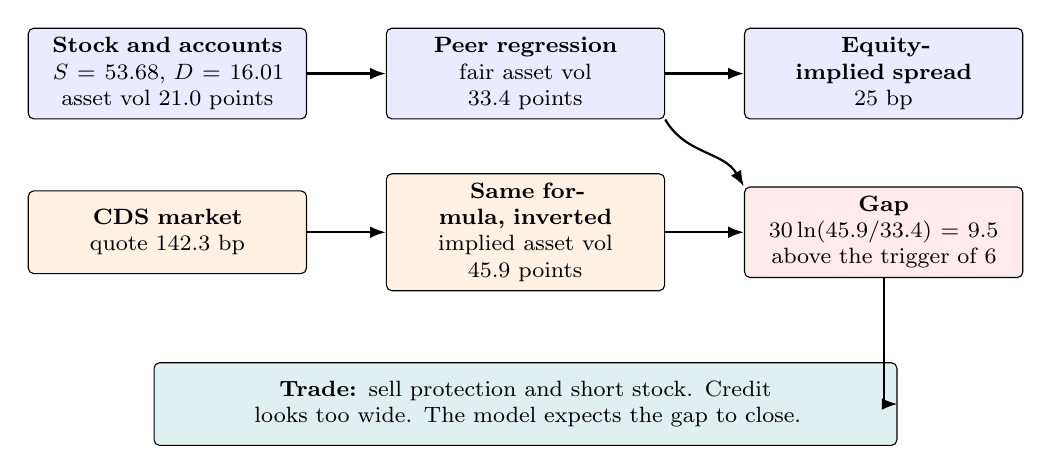
\begin{tikzpicture}[
  every node/.style={font=\footnotesize},
  b/.style={draw,rounded corners=2pt,align=center,text width=3.3cm,minimum height=1.05cm},
  a/.style={-{Latex[length=2mm]},thick}]
\node[b,fill=blue!8] (eq) at (0,0) {\textbf{Stock and accounts}\\$S=53.68$, $D=16.01$\\asset vol 21.0 points};
\node[b,fill=blue!8,right=1.0cm of eq] (fair) {\textbf{Peer regression}\\fair asset vol\\33.4 points};
\node[b,fill=blue!8,right=1.0cm of fair] (eqs) {\textbf{Equity-implied spread}\\25 bp};
\node[b,fill=orange!10,below=0.9cm of eq] (mk) {\textbf{CDS market}\\quote 142.3 bp};
\node[b,fill=orange!10,right=1.0cm of mk] (imp) {\textbf{Same formula, inverted}\\implied asset vol\\45.9 points};
\node[b,fill=red!8,right=1.0cm of imp] (gap) {\textbf{Gap}\\$30\ln(45.9/33.4)=9.5$\\above the trigger of 6};
\node[b,fill=teal!12,below=0.9cm of imp,text width=9.2cm] (tr) {\textbf{Trade:} sell protection and short stock. Credit looks too wide. The model expects the gap to close.};
\draw[a] (eq)--(fair); \draw[a] (fair)--(eqs); \draw[a] (mk)--(imp); \draw[a] (imp)--(gap);
\draw[a] (fair.south east) to[out=-60,in=120] (gap.north west);
\draw[a] (gap.south)|-(tr.east);
\end{tikzpicture}
\caption{The whole method on one real row: Altria (MO), 16 January 2004. Blue is the equity side. Orange is the credit side. The gap decides the trade. Section~\ref{sec:workbook} computes each number.}
\end{figure}

\begin{techbox}
Let $c$ be the market spread and $c^{*}$ the spread implied by equity. A method chooses a gap measure $g$ and a trigger $\tau$.
\[
g>\tau:\ \text{long credit, short stock.}\qquad g<-\tau:\ \text{short credit, long stock.}
\]
The three methods choose as follows.
\begin{center}\small
\begin{tabular}{@{}llll@{}}\toprule
Method & Credit leg & Gap $g$ & Trigger \\\midrule
Workbook & 5-year CDS & $30\ln(\sigma^{\text{imp}}/\sigma^{\text{fair}})$ & $\pm 6$, weekly \\
Yu on bonds & Bond & $\ln(z^{\text{mkt}}/z^{\text{model}})$ & $\ln(1+\alpha)$, $\alpha=0.5$, daily \\
Rank book (DES) & Bond and stock & $CS_D-CS_E$, in bp & Top and bottom quintile, monthly \\\bottomrule
\end{tabular}
\end{center}
Finkelstein's deck supplies an option-calibrated engine and no rule. Section~\ref{sec:fink} covers it.
\end{techbox}

\section{The shared engine: CreditGrades}\label{sec:engine}

\begin{plainbox}
\term{The picture.} Treat the firm's assets as a random walk. The firm defaults the first time its assets touch a barrier set by its debt. The barrier's height is uncertain, because nobody knows how much of the debt holders will recover until the default comes.

\term{What you put in and get out.} You put in the stock price, debt per share and asset volatility. You get out the chance of surviving to any date. That chance gives a fair CDS spread.

\term{Why it matters to you.} All your methods share this one formula. So they can share its errors. A disagreement between methods does not prove that one of them is right.

\term{New terms.} \term{Asset volatility} (asset vol) is how much the whole firm's value moves in a year. It sits below equity vol, because debt magnifies moves in the stock. A \term{basis point} (bp) is 0.01\%.
\end{plainbox}

\begin{techbox}[Equations and code]
\textbf{Symbols.} $S$ stock price. $D$ debt per share. $\bar L$ mean barrier as a share of debt. $\lambda$ uncertainty of the barrier. $\sigma_A$ asset vol. $\sigma_S$ equity vol. $T$ maturity. $r$ risk-free rate. $R$ recovery. $\Phi$ the standard normal distribution function.

\textbf{Asset vol from equity vol.}
\[
\sigma_A=\sigma_S\,\frac{S}{S+\bar L D}
\]
\textbf{Survival.} Set
\[
d=\Bigl(1+\frac{S}{\bar L D}\Bigr)e^{\lambda^2},\qquad a(t)=\sqrt{\sigma_A^2 t+\lambda^2},
\]
\[
B(d,a)=\Phi\!\Bigl(\frac{\ln d}{a}-\frac a2\Bigr)-d\,\Phi\!\Bigl(-\frac{\ln d}{a}-\frac a2\Bigr).
\]
Survival to $t$ is $B(d,a(t))$. Note that $B(d,\lambda)<1$. The firm has some chance of being past the barrier today, because the barrier is uncertain.

\textbf{CDS spread.} Set $z=\sqrt{\tfrac14+2r/\sigma_A^2}$ and
\[
G(d,x,z)=d^{z+\frac12}\Phi\!\Bigl(-\frac{\ln d}{x}-zx\Bigr)+d^{\frac12-z}\Phi\!\Bigl(-\frac{\ln d}{x}+zx\Bigr),
\]
\[
H(T)=e^{r(\lambda/\sigma_A)^2}\bigl[G(d,a(T),z)-G(d,\lambda,z)\bigr].
\]
\[
c(T)=\frac{360}{365}\,(1-R)\,\frac{1-B(d,\lambda)+H(T)}{\bigl[B(d,\lambda)-B(d,a(T))e^{-rT}-H(T)\bigr]/r}.
\]
\textbf{Settings.} Workbook: $\bar L=0.5$, $\lambda=0.3$, $R=0.4$, $T=5$, $r$ the 5-year swap rate. Yu: $\lambda=0.3$, $R=0.5$, with $\bar L$ fitted.

\textbf{Code.} \fn{_b}, \fn{_g}, \fn{_terms}, \fn{model_spread}, \fn{implied_asset_vol} in \fn{e2c_model.py}. \fn{survival} and \fn{cds_par_spread} in \fn{e2c_bond.py}. \fn{fk_survival} in \fn{fk_model.py} is the same survival formula with a shifted barrier $B=\bar L D$.
\end{techbox}

\begin{figure}[H]
\centering
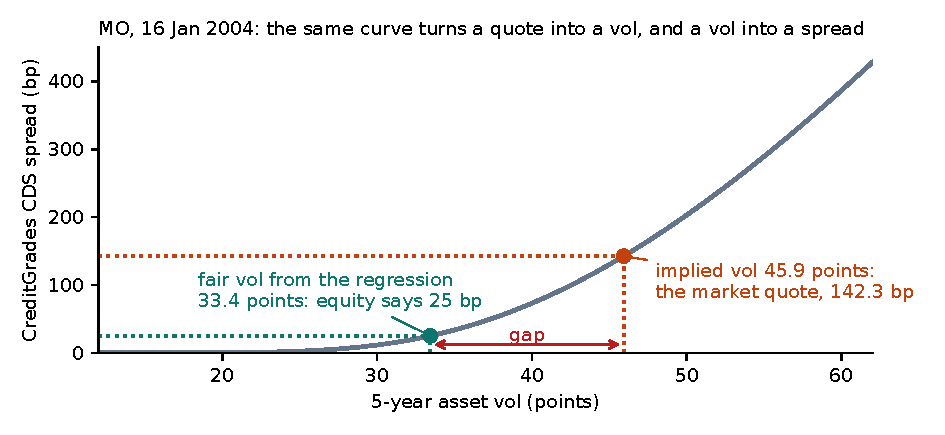
\includegraphics[width=0.92\linewidth]{inversion.pdf}
\caption{One curve, read in both directions. Read up from a vol to get a spread. Read across from a quote to get a vol. The curve is steep at high vol and flat near zero, so a spread gap and a vol gap do not measure the same thing.}
\end{figure}

\section{The workbook method}\label{sec:workbook}

\begin{plainbox}
\term{What it is.} This is your own 2005 model, rebuilt in Python. It runs every Friday on a list of names with 5-year CDS. It has eight steps.
\begin{enumerate}[leftmargin=1.4em,nosep]
\item Turn the balance sheet into debt per share.
\item Average several equity vols and convert them to asset vol. Call this the \term{historical} vol.
\item Find the asset vol that makes the formula match the CDS quote. Call this the \term{implied} vol.
\item Compare implied with historical across all names that week. The ratio changes with leverage, so fit a line through the cross-section.
\item Use that line to get each name's \term{fair} vol.
\item Compute the gap between implied and fair. This is the \term{residual}.
\item Trade if the residual passes $\pm 6$. Size the trade so a 3-point move earns a fixed dollar amount.
\item Hedge with stock, mark to the next week, and rebuild the book.
\end{enumerate}

\term{Why it matters to you.} This is the only method with real data behind it. It gives the 2.51 Sharpe. It rebuilds the workbook: the repository logs 11,465 comparisons with no failures.

\term{The catch.} The model compares each name with its peers that week. So it asks ``rich against peers'', not ``rich against the true value''.
\end{plainbox}

\begin{techbox}[Equations and code, in \fn{e2c_model.py}]
\textbf{S01 Debt per share} (\fn{debt_per_share}). The $0.5$ weight treats half of other liabilities as debt.
\[
F=\text{st}+\text{lt}+0.5(\text{other}_{st}+\text{other}_{lt}),\quad k_0=\min(\text{minority},0.5F),\quad k_1=\min(\text{pref},0.5\,\text{mcap}),
\]
\[
D=\frac{F-k_0}{(\text{mcap}+k_1)/S}.
\]
\textbf{S02, S03 Vols} (\fn{average_equity_vol}, \fn{historical_asset_vol}). The equity vol is the plain average of the 30, 60, 90, 180 and 360-day realised vols and the 3, 6, 12 and 24-month put vols. Then $\sigma^{\text{hist}}=\sigma_S\,S/(S+0.5D)$.

\textbf{S06 Implied vol} (\fn{implied_asset_vol}). Solve $c(5;\sigma^{\text{imp}})=c^{\text{mkt}}$.

\textbf{S07 Regression} (\fn{leverage_regression}). On each date, across all names,
\[
\ln\frac{\sigma_i^{\text{imp}}}{\sigma_i^{\text{hist}}}=\ln w_t+\beta_t\ln\frac{S_i}{D_i}+\epsilon_i.
\]
\textbf{S08 Fair vol} (\fn{fair_asset_vol}). With $p=0.95$, prior coefficient $1$ and prior skew $0$,
\[
\sigma_i^{\text{fair}}=\sigma_i^{\text{hist}}\Bigl[p\,w_t(S_i/D_i)^{\beta_t}+(1-p)\Bigr].
\]
\textbf{S09 Residual} (\fn{vol_residual}). $\;e_i=30\ln(\sigma_i^{\text{imp}}/\sigma_i^{\text{fair}})$.

\textbf{S11 Signal} (\fn{trade_signal}). $e_i>6$: sell protection, short stock. $e_i<-6$: buy protection, long stock.

\textbf{S13 Size} (\fn{trade_size}). $\nu$ is the CDS value change per vol point, $Q$ the notional in \$M. The 3-point target earns \$0.2M, with a \$10M limit.
\[
Q=\min\Bigl(10,\ \frac{0.2}{|\nu|\cdot 3\cdot \sigma^{\text{imp}}/30}\Bigr).
\]
\textbf{S14 Hedge} (\fn{equity_hedge}). Stock hedge in \$M is $Q\Delta$, with $\Delta$ from \fn{cds_greeks}.

\textbf{S15 P\&L} (\fn{weekly_pnl}), in \$ thousands, for sold protection. $A$ is the risky annuity, $\delta$ the days to the next row, $\rho$ the stock return.
\[
\underbrace{-Q\,\Delta c\,A/10}_{\text{spread}}\;\underbrace{-\,Q\Delta\,\rho\cdot 1000}_{\text{stock}}\;\underbrace{+\,Q\,(c/10)\,\delta/360}_{\text{carry}}\;\underbrace{+\,Q\Delta\,(r-0.5\%)\,\delta/360\cdot 1000}_{\text{short rebate}}.
\]
A purchase of protection flips the signs and pays $r+0.5\%$ on the long stock.
\end{techbox}

\begin{examplebox}{Worked example on a real row: MO, 16 January 2004 (the row \fn{05_io_spec.md} uses)}
\begin{center}\small
\begin{tabular}{@{}p{3.2cm}p{7.2cm}r@{}}\toprule
Step & Computation & Result\\\midrule
Debt per share & $F=3376+21163+0.5(14819+10672)=37284.5$. $k_0=4760$. $k_1=0$. Shares $=109033.3/53.68$ & $D=16.01$\\
Equity vol & Average of the nine vols & 24.10\\
Historical asset vol & $24.10\times 53.68/(53.68+8.01)$ & 20.97\\
Implied asset vol & Solve the formula at 142.3 bp, $r=3.41\%$ & 45.94\\
Regression that date & $w_t=1.1409$, $\beta_t=0.2929$. $S/D=3.352$ & \\
Fair vol & $20.97\,[0.95\times1.1409\times3.352^{0.2929}+0.05]$ & 33.44\\
Residual & $30\ln(45.94/33.44)$ & 9.52\\
Signal & $9.52>6$ & sell protection\\
Size & $\nu=0.00627$. $\;0.2/(0.00627\times3\times45.94/30)$ & \$6.94M\\
Stock hedge & $6.94\times\Delta$, with $\Delta=0.1025$ & \$0.711M short\\\midrule
Spread leg & 142.33 to 136.25 bp, $A=4.510$ & $+19.04$\\
Stock leg & 53.68 to 54.48, a loss on the short & $-10.60$\\
Carry, 7 days & $6.94\times14.233\times7/360$ & $+1.92$\\
Short rebate & $0.711\times(3.41\%-0.5\%)\times7/360\times1000$ & $+0.40$\\
\textbf{Week's P\&L} & \$ thousands & $\mathbf{+10.76}$\\\bottomrule
\end{tabular}
\end{center}
\term{Read it this way.} The credit tightened and earned money. The stock rose, so the hedge lost part of it. One good week proves nothing. It only shows the arithmetic.
\end{examplebox}

\begin{examplebox}{Whole-panel result, from \fn{run_pipeline}}
19,489 rows, 170 names, 151 Fridays from 27 September 2002 to 23 September 2005. Gross Sharpe 2.51, annual return 20.6\%, annual vol 8.2\%, worst drawdown 3.6\%, $t=4.28$. These equal the workbook's cells. They count no trading costs and assume you trade at the signal's own close.
\end{examplebox}

\section{Yu's method on bonds}\label{sec:yu}

\begin{plainbox}
\term{What it is.} Fan Yu (2005) tested the same idea on CDS. Your files have no bond version, so the repository adapts Yu to bonds. The bond's market spread takes the place of the CDS quote.

\term{The main differences from the workbook.}
\begin{itemize}[leftmargin=1.2em,nosep]
\item It compares each name with its own model value. It does not compare it with peers that week.
\item It fits one number for each name, the barrier, on the first days of data. It then freezes that number. So the first days set the ``normal'' gap for that name.
\item It checks every day and enters when market and model differ by a set ratio.
\item It exits when the two meet, when the holding period ends, or when the position's value goes negative.
\end{itemize}

\term{Why it matters to you.} Bonds are what you can compare with the published bond results. But a bond also carries interest-rate risk and has thinner trading, so this method adds a Treasury hedge and trade cleaning.

\term{New terms.} A \term{Z-spread} is the constant spread over the Treasury zero curve that prices the bond's cash flows at its market price.
\end{plainbox}

\begin{techbox}[Equations and code, in \fn{e2c_bond.py}]
\textbf{Market spread} (\fn{z_spread}). Solve $P^{\text{full}}=\sum_i CF_i\,DF(t_i)\,e^{-z t_i}$ for $z^{\text{mkt}}$.

\textbf{Model price} (\fn{risky_bond_price}), an adaptation. Recovery $R_b=0.5$ of face is paid at default.
\[
P^{\text{model}}=\sum_i CF_i\,DF(t_i)\,q(t_i)+R_b\Bigl(1-q(0)+\int_0^{T}DF(s)\bigl(-q'(s)\bigr)\,ds\Bigr).
\]
Solving the Z-spread equation on $P^{\text{model}}$ gives $z^{\text{model}}$ (\fn{model_z_spread}).

\textbf{Barrier fit} (\fn{calibrate_barrier}, \fn{fit_barrier_on_bond}). Choose one $\bar L$ by least squares on the spread over the first days. Yu uses 10 days of CDS. The bond default is 20.
\[
\hat{\bar L}=\arg\min_{\bar L}\sum_{t\le 20}\bigl(z_t^{\text{model}}(\bar L)-z_t^{\text{mkt}}\bigr)^2.
\]
\textbf{Signal} (\fn{entry_signal}, Yu Eq.~8). $\alpha=0.5$ by default.
\[
z^{\text{mkt}}>(1+\alpha)z^{\text{model}}\Rightarrow\text{long bond, short stock.}\qquad z^{\text{model}}>(1+\alpha)z^{\text{mkt}}\Rightarrow\text{short bond, long stock.}
\]
\textbf{Legs} (\fn{build_position}). Stock hedge per 1 of face is $\partial P^{\text{model}}/\partial S$ (\fn{bond_equity_delta}), holding asset vol fixed. A Treasury hedge matches dollar duration (\fn{rate_hedge_face}).

\textbf{Exits} (\fn{exit_reason}, \fn{bond_exit_reason}). Value below zero, convergence, end of the 180-day hold, plus forced events. Capital is 0.5 per 1 of notional, and execution lags the signal by one day (\fn{BacktestConfig}).

\textbf{Additions beyond Yu.} Trade cleaning, a peer adjustment, a sibling and CDS veto, a cost gate. The file tags these [ADAPTATION]. \fn{run_bond_backtest} is the entry point, and \fn{run_yu.py} is the one-command runner.
\end{techbox}

\begin{examplebox}{Worked example. ALL INPUTS ARE MADE UP (\fn{worked_example.py})}
A made-up 5.5\% bond with 4.8 years left, and a made-up issuer.
\begin{enumerate}[leftmargin=1.4em,nosep]
\item Fit: 20 days with market Z near 171 bp give $\bar L=0.8410$, with a fit error of 2.3 bp.
\item Later, the bond sells off. Market Z is 329.9 bp and model Z is 197.0 bp.
\item The ratio is $1.674$, above $1.5$. The signal is long bond, short stock, short Treasury.
\item Good path: net $+8.69\%$ on capital. Bad path, same entry: net $-21.04\%$ on capital.
\end{enumerate}
\term{Read it this way.} The author chose both paths. The example shows the arithmetic and gives no evidence on the trade.
\end{examplebox}

\section{Finkelstein: options join in}\label{sec:fink}

\begin{plainbox}
\term{What it is.} Finkelstein's 2002 deck uses the same structural idea and calibrates it to equity options. Options set the asset vol at each maturity. The same model then prices stock, options, CDS and bonds.

\term{What is new.}
\begin{itemize}[leftmargin=1.2em,nosep]
\item A put on a risky stock is partly default insurance. So the put market holds its own view of credit.
\item With three markets you get three gaps. Two of them are independent. They can say \emph{which} market is out of line.
\item Because one model prices everything, you can solve a hedge against stock moves, vol moves and default at once.
\end{itemize}

\term{Important.} The deck gives no arbitrage signal and no trading rule. It has no entry, exit, sizing, costs or backtest. Every trading rule built on it in this repository is an addition, and the code tags these [ADAPTATION].

\term{Why it matters to you.} Agreement across markets is the best untested idea for picking names better. It needs dated option quotes, which the old panel does not have.

\term{State of the code.} The model, values and hedge work are coded and tested against the deck's numbers. No option adapter or runner exists yet.
\end{plainbox}

\begin{techbox}[Equations and code, in \fn{fk_model.py}, \fn{fk_value.py}, \fn{fk_risk.py}]
\textbf{Shifted lognormal stock with a knock-out.} Assets $V$ have zero drift and start at $S_0+B$. The stock is
\[
S_t=(V_t-B)\,e^{(r-p)t}
\]
until $V$ touches the barrier $B$. After that the stock is zero.

\textbf{Survival} (\fn{fk_survival}). With no barrier uncertainty,
\[
Q(T)=\Phi\!\Bigl(\frac{\ln d}{A}-\frac A2\Bigr)-d\,\Phi\!\Bigl(-\frac{\ln d}{A}-\frac A2\Bigr),\quad d=\frac{S_0+B}{B},\quad A=\sigma(T)\sqrt T.
\]
With uncertainty $\lambda$, $d$ gains a factor $e^{\lambda^2}$ and $A^2$ gains $\lambda^2$.

\textbf{Vol term structure} (\fn{forward_vol}, \fn{flat_forward_sigma}, \fn{equity_vol_from_asset}). Option vols at each expiry give the cumulative asset vol $\sigma(T)$, using $\sigma_S=\sigma_A(S+B)/S$. Forward vol between two expiries is $\sqrt{(\sigma_2^2T_2-\sigma_1^2T_1)/(T_2-T_1)}$.

\textbf{Put} (\fn{fk_put}). The deck prints no put formula. The code derives one from the reflection principle.
\[
\text{put}=\underbrace{K e^{-rT}\bigl(1-Q(T)\bigr)}_{\text{default part}}+\underbrace{e^{-pT}\Bigl[G(V_0)-\frac{V_0}{B}G\bigl(B^2/V_0\bigr)\Bigr]}_{\text{diffusion part}},
\]
where $G(x)=E[(H-V_T)^+;\,V_T>B]$ for lognormal $V_T$ from $x$, $V_0=S_0+B$ and $H=B+Ke^{-(r-p)T}$.

\textbf{Three gaps} (\fn{three_gaps}), an adaptation. $z_m$ is the market bond spread, $z_o$ the option-implied model spread, $z_s$ the stock-only model spread.
\[
G_{bp}=\ln\frac{z_m}{z_o},\qquad G_{ps}=\ln\frac{z_o}{z_s},\qquad G_{bs}=\ln\frac{z_m}{z_s}=G_{bp}+G_{ps}.
\]
\textbf{Hedge} (\fn{solve_hedge}). Pick a row for each hedge leg from delta, vega and jump. Solve $Mn=-g$, where $g$ holds the target's sensitivities and $M$ the legs'. The guards reject a short option and a very large stock position. Those guards are additions.
\end{techbox}

\begin{figure}[H]
\centering
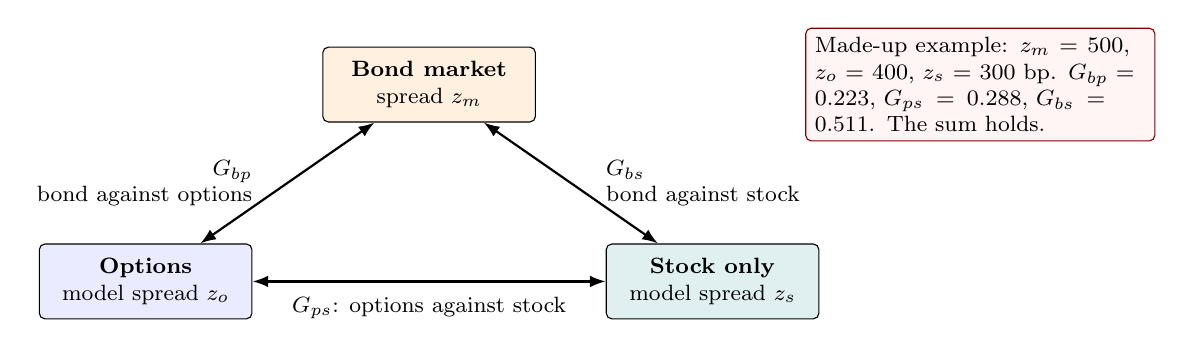
\begin{tikzpicture}[every node/.style={font=\footnotesize},
  m/.style={draw,rounded corners=2pt,align=center,minimum width=2.7cm,minimum height=0.95cm},
  e/.style={{Latex[length=2mm]}-{Latex[length=2mm]},thick}]
\node[m,fill=orange!12] (b) at (0,2.5) {\textbf{Bond market}\\spread $z_m$};
\node[m,fill=blue!8] (o) at (-3.6,0) {\textbf{Options}\\model spread $z_o$};
\node[m,fill=teal!12] (s) at (3.6,0) {\textbf{Stock only}\\model spread $z_s$};
\draw[e] (b)--node[left=9pt,align=right]{$G_{bp}$\\bond against options} (o);
\draw[e] (b)--node[right=9pt,align=left]{$G_{bs}$\\bond against stock} (s);
\draw[e] (o)--node[below=2pt,align=center]{$G_{ps}$: options against stock} (s);
\node[align=left,draw=red!50!black,fill=red!4,rounded corners=2pt,text width=4.2cm] at (7.0,2.5) {Made-up example: $z_m=500$, $z_o=400$, $z_s=300$ bp. $G_{bp}=0.223$, $G_{ps}=0.288$, $G_{bs}=0.511$. The sum holds.};
\end{tikzpicture}
\caption{Three markets, three gaps, two independent. If only $G_{bp}$ is large, the bond looks out of line. If only $G_{ps}$ is large, the bond and options agree against the stock.}
\end{figure}

\begin{figure}[H]
\centering
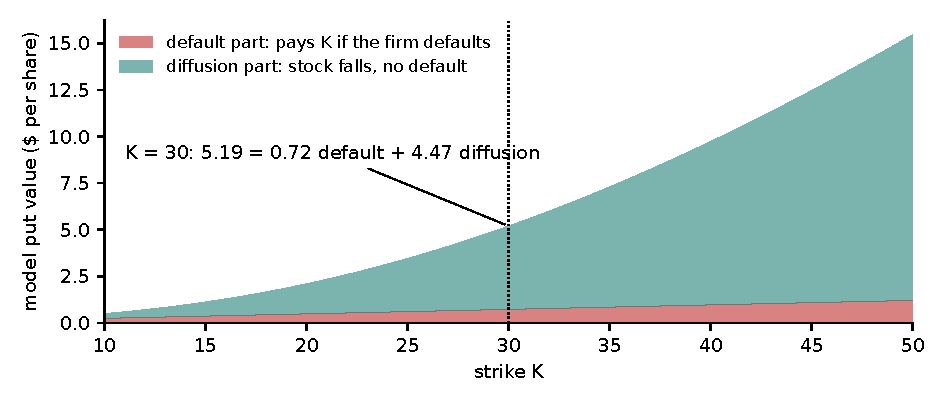
\includegraphics[width=0.92\linewidth]{put_split.pdf}
\caption{A put splits into two parts, from \fn{fk_put}. The setting is that of slides 21--25: $S=40$, $B=15$, $\sigma=0.375$, $r=5\%$, $p=2\%$, two years. The deck quotes this put at 5.22, and the code computes 5.19.}
\end{figure}

\begin{examplebox}{Worked hedge from the deck's setting (\fn{fk_risk.py}, per \$100 protection sold)}
Sell \$100 of 5-year protection at 560 bp with $R=10\%$. Hedge with the $K=30$ two-year put at 5.22 and with stock. Protect against stock moves and against a sudden default.
\begin{center}\small
\begin{tabular}{@{}lrrr@{}}\toprule
 & Delta & Jump & Vega\\\midrule
Protection sold & $+0.657$ & $-90.00$ & $-53.29$\\
One put & $-0.227$ & $+21.93$ & $+8.64$\\\midrule
Hedge: 4.96 puts (\$25.89) and 0.469 shares (\$18.76) & & & \\
Net after the hedge & 0 & 0 & $-10.44$\\\bottomrule
\end{tabular}
\end{center}
\term{Three things to notice.} The stock position is long, not short. Most of the default protection comes from puts. Vega is left over, because two legs can only cancel two risks.

\term{A convention to know.} This table leaves the contract's own value out of the jump, which is the code's default and fits the deck's slides best. Setting \fn{include_value=True} gives a jump of $-95.51$, then 5.39 puts and 0.566 shares. The note \fn{model_analysis_and_improvements} quotes that version.

\term{Deck numbers.} Slide 1 says a put splits 1.90 of 4.92 at the money and 1.42 of 2.72 at 30\% out of the money. Those values do not all reproduce from the slide's own inputs. The plan lists the differences.
\end{examplebox}

\section{The debt-equity spread and F10}\label{sec:f10}

\begin{plainbox}
\term{What it is.} Chen, Chen and Li (2026, \emph{Journal of Finance}) measure the gap between a bond's actual spread and its equity-implied spread. They call it the debt-equity spread (DES). Each month they rank firms into five groups. Bonds in the top group, the widest against equity, then outperform. Stocks in that group underperform.

\term{What F10 is.} F10 is an acceptance test in the plan. It asks: on your data, do you see the published pattern? It is the first test that needs real data and no options.

\term{Why it matters to you.} It gives an outside benchmark. If your data and code cannot show the published signs, you stop and debug before any option work.

\term{Important.} No copy of the paper is in this repository's working files. The published figures and definitions below come from the plan's notes on it. So a miss may reflect a definition gap and not a failed idea.

\term{State of the code.} This section describes commit \fn{784361b} on branch \fn{method/f10}. That work was still running when this was written. F10 has not run on real data, so it has no result.
\end{plainbox}

\begin{techbox}[Equations and code, in \fn{fk_des.py}, \fn{fk_f10.py}, \fn{run_f10.py}]
\textbf{The gap} (\fn{bond_des}). Each spread is a yield less the yield of a synthetic Treasury with the same cash flows. The Treasury cancels.
\[
\text{DES}=CS_D-CS_E=y(P^{\text{mkt}})-y(P^{\text{equity model}}).
\]
\textbf{Equity model} (\fn{des_survival}). Extended CreditGrades. Assets drift at $r-\delta$, and barriers above today's assets are cut off. $\bar L=0.5$, $\lambda=0.3$, recovery $0.35$ of face.

\textbf{Inputs} (\fn{payout_delta}, \fn{rolling_equity_vol}, \fn{accounts_asof}). Payout $\delta$ is dividends, interest and repurchases over the sum $S+D$ per share, capped at 15\%. Vol is 3-year realised. Accounts lag at least two months.

\textbf{Firm and rank} (\fn{firm_des}, \fn{quintile_sort}). Average DES across a firm's bonds, weighted by lagged bond value. Sort into quintiles each month.

\textbf{Book} (\fn{t0_returns}). Long top-group bonds, short bottom-group bonds. Long bottom-group stocks, short top-group stocks. Holds of 1, 3 and 6 months. Each leg is reported apart.

\textbf{Added for F10.} Bond screens with a funnel (\fn{screen_bonds}). Financing and borrow fees (\fn{financing_drag}). A Treasury overlay (\fn{overlay_series}). Splits by bond size and fee (\fn{median_split}). The plan's stop rule on large bonds (\fn{stop_rule}). Newey--West $t$-statistics with 6 lags (\fn{newey_west}).

\textbf{Point in time.} \fn{run_f10.py} builds each month's inputs as known at the end of that month (\fn{build_vintage_inputs}). A later correction cannot reach an earlier sort.
\end{techbox}

\begin{techbox}[The test]
\textbf{Published targets, from the plan.} These are gross. Window for the main test is January 2002 to December 2021, value-weighted, 1-month hold.
\begin{center}\small
\begin{tabular}{@{}ll@{}}\toprule
Bond premium, full sample & 5.28\% a year, $t=5.64$\\
Bond premium, clean returns, 2002--2021 & 3.24\% a year, $t=2.69$\\
Stock premium & 6.56\% a year, $t=3.79$\\
Quintile gaps, Q1 to Q5 & $-139$ to $+271$ bp\\
Price ratio, Q1 to Q5 & 0.94 to 1.16\\\bottomrule
\end{tabular}
\end{center}
\textbf{The plan's rule.} ``Signs must match. Sizes as shape, if samples differ.'' So: Q1 gap below 0, Q5 gap above 0, Q1 ratio below 1, Q5 ratio above 1, bond premium above 0, stock premium above 0.

\textbf{Rules added in \fn{fk_f10.py}, written before any real data was seen.}
\begin{enumerate}[leftmargin=1.4em,nosep]
\item The bond premium also needs $t\ge 1.96$, because a sign on noise is no reproduction.
\item NOT JUDGED below 60 months or a median of 25 sorted firms.
\item Both continuous and semiannual yields run. You have not chosen, so the overall verdict is the weaker of the two.
\item The size gap to 3.24\% is reported and does not decide the verdict.
\end{enumerate}
\textbf{Verdicts.} REPRODUCED, NOT REPRODUCED, or NOT JUDGED with a reason.
\end{techbox}

\begin{warnbox}{What a REPRODUCED verdict would not mean}
It means the signs match on your sample. It does not mean you could earn 3.24\%. The published figures are gross, and the plan's stop rule looks at the net return on large bonds. A clean result still depends on the point-in-time data and on dead names being in the universe.
\end{warnbox}

\section{Selecting names: the hold band and the cap}\label{sec:select}

\begin{plainbox}
\term{The problem.} The workbook rebuilds its book every Friday. A name that drifts from 6.1 to 5.9 leaves the book, and it may come back next week. Each round trip pays the spread. At a 5\% round-trip cost, costs take most of the return.

\term{The hold band.} Enter past 6. Stay in until the gap falls to 3. This stops the churn from small wobbles around the trigger.

\term{The cap.} Hold at most 20 names on each side. Fill free slots with the names that have the highest expected gain per dollar of cost.

\term{What we learned.}
\begin{itemize}[leftmargin=1.2em,nosep]
\item The hold band roughly doubles the Sharpe after costs, from 0.55 to 1.15.
\item The cap keeps about half the names, at a Sharpe of 0.96. That is lower than the band alone, and five names matter more.
\item A bigger gap does not pick next week's winners. The ranking works by avoiding cost.
\end{itemize}

\term{Why it matters to you.} The band is the base case. The cap is the alternative to compare on real data. Both are off by default, so the workbook's 2.51 still reproduces.
\end{plainbox}

\begin{figure}[H]
\centering
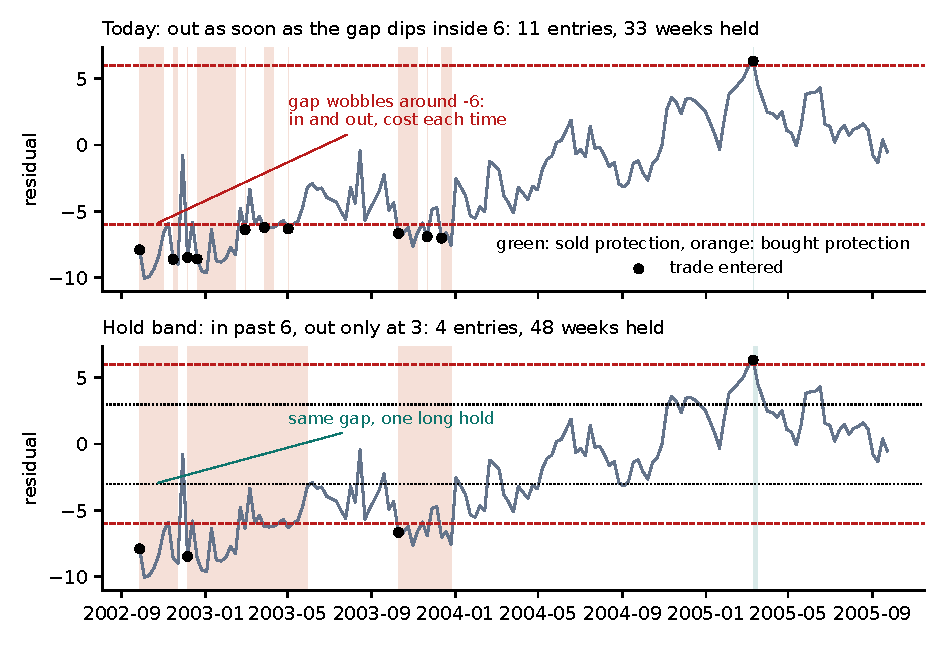
\includegraphics[width=0.92\linewidth]{hold_band.pdf}
\caption{Before and after on one real name, GE. Each dot is a new trade, and each one pays the cost. Shading shows when a position is on. Today it enters 11 times over 33 weeks held. The band enters 4 times over 48 weeks held. I picked GE because the band changes it most among names with trades on both sides, so it shows the rule and is not typical.}
\end{figure}

\begin{techbox}[Rules and code, in \fn{e2c_model.py}, step S11a]
\textbf{Hold band} (\fn{held_signal}, \fn{Params.exit_trigger}). Side $s=\pm1$.
\[
\text{enter if } s\,e_{i,t}>6,\qquad\text{stay while } s\,e_{i,t}>3.
\]
A week with no row keeps the position. A blank residual or an out-of-range spread closes it.

\textbf{Cap} (\fn{Params.max_per_side}). Held names keep their slots. New names fill free slots by
\[
\frac{\text{gain}}{\text{cost}}=\frac{|\nu|\,(\sigma^{\text{imp}}/30)\,|e_i|}{A\,(c/10^4)\,b},\qquad b=5\%\ \ (\fn{gain_per_cost}).
\]
Notional cancels, so the rank does not depend on the size limit.

\textbf{Cost} (\fn{trading_cost}). For each change in signed size, in \$ thousands,
\[
|\Delta Q|\cdot 1000\cdot A\cdot(c/10^4)\cdot b/2.
\]
It covers CDS only. It has no stock cost and no execution lag, and the last open position pays no exit cost.
\end{techbox}

\begin{figure}[H]
\centering
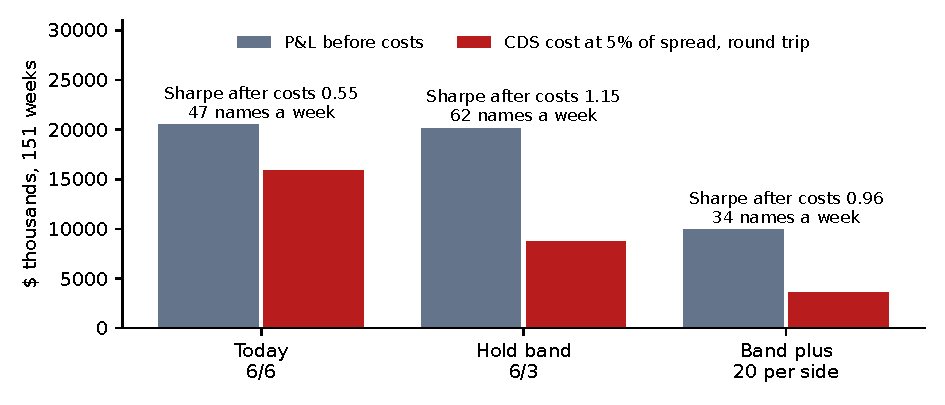
\includegraphics[width=0.92\linewidth]{costs.pdf}
\caption{Where the money goes. The band gives up almost no P\&L before costs and pays about half the cost. The cap roughly halves the P\&L and cuts the cost by about 60\%.}
\end{figure}

\begin{examplebox}{The numbers. All in-sample, on survivors, 151 weeks, cost 5\% of spread}
\begin{center}\small
\begin{tabular}{@{}lrrrrrr@{}}\toprule
Book & Names & P\&L & Cost & Sharpe, raw & Sharpe, NAV & Top 5 share\\\midrule
Today, 6/6 & 47 & 20,478 & 15,870 & 0.55 & 0.57 & 37\%\\
Hold band, 6/3 & 62 & 20,145 & 8,711 & 1.15 & 1.15 & 36\%\\
Band plus 20 per side & 34 & 9,898 & 3,570 & 0.96 & 1.04 & 51\%\\\bottomrule
\end{tabular}
\end{center}
P\&L and cost are in \$ thousands. Names is the average held per week.

\term{Two Sharpe bases.} ``Raw'' uses the weekly dollar P\&L after cost. ``NAV'' divides by the week's NAV, the workbook's own return, and \fn{run_workbook.py} reports this one. The gross figures are 2.49 raw and 2.51 NAV for today's book. Compare a number only with one on the same basis.

\term{A correction.} I first reported 1.15 for the capped book. That ranking gave every trade the full target gain. About 80\% of trades sit at the \$10M limit, so they cannot reach the target and the ranking overstated them. The corrected formula gives 0.96. The old ranking reproduces 1.15 raw, with a top-5 share of 47\%.
\end{examplebox}

\begin{techbox}[Three checks, computed by \fn{make_figs.py}]
\textbf{Does gap size pick winners?} Among names past the trigger, the mean weekly rank correlation of $|e_i|$ with next week's P\&L is 0.004, with $t=0.31$. So it does not.

\textbf{Does the cap beat chance?} Twenty runs that fill the cap's slots at random give raw Sharpes from 0.38 to 0.89, with a mean of 0.64. The ranked book's 0.96 sits above all twenty. It sits below the uncapped band at 1.15. This run replaces an earlier one with a range of 0.47 to 0.86, which used the first ranking's study script and other random draws.

\textbf{Is the book only riding the market?} I regressed weekly P\&L on the panel's mean stock return and median spread change, with Newey--West errors over 4 lags. About 85\% of the mean P\&L remains unexplained, and the Sharpe after removing these moves is 2.17. Each side alone is about half market risk ($R^2$ 0.50 and 0.58). What remains is significant for short credit ($t=2.57$) and not for long credit ($t=1.21$). The two sides offset, so the check needs a balanced book. The market measures come from the panel's own survivors.
\end{techbox}

\begin{warnbox}{How much to trust this}
I tried many rules on the same 151 weeks. Fix a rule before you see new data, and do not pick the best row. A rule that wins here can lose on real data with dead names and filing dates.
\end{warnbox}

\section{The data layer}\label{sec:data}

\begin{plainbox}
\term{The problem.} Your production data sits on another machine, and this public repository must not hold it. The methods also must not see data before it was public.

\term{The answer.} All data passes through one small door, a single \fn{read} function. Your production code stays off this repository and only has to answer that one call. A \term{view} stands between the data and the methods and shows only what was known at a chosen time.

\term{Why it matters to you.} You can plug in production data by changing one setting, without changing any method. You can export files or write a small adapter. A check then runs first and tells you what is wrong with the data.

\term{New terms.} \term{Point-in-time} means as it was known on that date. \term{Look-ahead} is the error of using something before it was public. A \term{restatement} is a later correction to reported numbers.
\end{plainbox}

\begin{figure}[H]
\centering
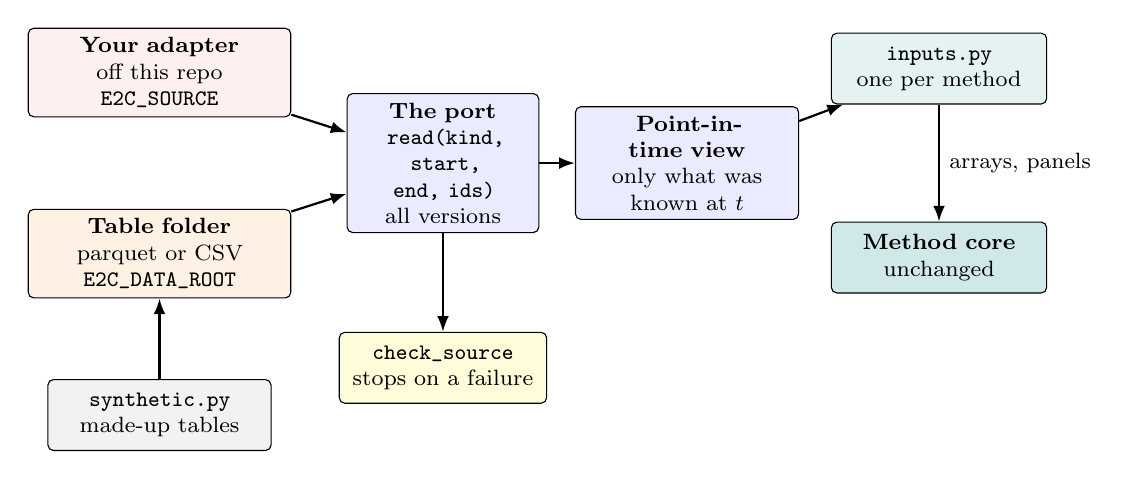
\begin{tikzpicture}[every node/.style={font=\footnotesize},
  b/.style={draw,rounded corners=2pt,align=center,minimum height=0.9cm},
  a/.style={-{Latex[length=2mm]},thick}]
\node[b,fill=red!6,text width=3.1cm] (prod) at (0,1.15) {\textbf{Your adapter}\\off this repo\\\fn{E2C_SOURCE}};
\node[b,fill=orange!10,text width=3.1cm] (tab) at (0,-1.15) {\textbf{Table folder}\\parquet or CSV\\\fn{E2C_DATA_ROOT}};
\node[b,fill=blue!8,text width=2.2cm] (port) at (3.6,0) {\textbf{The port}\\\fn{read(kind, start, end, ids)}\\all versions};
\node[b,fill=blue!8,text width=2.6cm] (view) at (6.7,0) {\textbf{Point-in-time view}\\only what was known at $t$};
\node[b,fill=teal!10,text width=2.5cm] (ad) at (9.9,1.2) {\textbf{\fn{inputs.py}}\\one per method};
\node[b,fill=teal!18,text width=2.5cm] (core) at (9.9,-1.2) {\textbf{Method core}\\unchanged};
\node[b,fill=yellow!15,text width=2.4cm] (chk) at (3.6,-2.6) {\textbf{\fn{check_source}}\\stops on a failure};
\node[b,fill=gray!10,text width=2.6cm] (syn) at (0,-3.2) {\textbf{\fn{synthetic.py}}\\made-up tables};
\draw[a] (prod)--(port); \draw[a] (tab)--(port); \draw[a] (port)--(view);
\draw[a] (view)--(ad); \draw[a] (ad)--node[right]{arrays, panels}(core);
\draw[a] (port)--(chk); \draw[a] (syn)--(tab);
\end{tikzpicture}
\caption{The flow. Sources sit on the left. Methods sit on the right. The method core knows nothing about where data comes from.}
\end{figure}

\begin{techbox}[Interfaces and code, in \fn{e2c_data/}]
\textbf{Port} (\fn{source.py}). Any object with this method is a source. It returns every version it holds.
\begin{center}\small \fn{read(kind, start=None, end=None, ids=None) -> DataFrame}\end{center}
\textbf{View} (\fn{view.py}). \fn{PointInTimeView(source, decision_time)} has three reads.
\begin{itemize}[leftmargin=1.2em,nosep]
\item \fn{read}: the latest version of each row known at the decision time.
\item \fn{versions}: every version known at the decision time. A backtest needs this for accounts, or restated numbers would reach earlier dates.
\item \fn{issuers_on}: dated instrument-to-issuer links. Two issuers at once raises an error.
\end{itemize}
A read past the decision time raises \fn{LookAheadError}. A missing kind raises \fn{DataUnavailable}. Missing values stay NaN, never zero.

\textbf{15 kinds} (\fn{schema.py}). Each carries \fn{available_at}, the moment it became public.
\begin{center}\small
\begin{tabular}{@{}ll@{}}\toprule
Identity & \fn{security_map}, \fn{universe}, \fn{issuer_attributes}\\
Equity & \fn{equity_prices}, \fn{corporate_actions}\\
Accounts & \fn{accounts}\\
Rates, funding & \fn{rates}, \fn{financing}\\
Credit & \fn{cds_quotes}, \fn{bond_terms}, \fn{bond_prices}, \fn{bond_trades}\\
Options, events, factors & \fn{option_quotes}, \fn{events}, \fn{factor_returns}\\\bottomrule
\end{tabular}
\end{center}
\textbf{Units.} Rates, spreads and vols are decimals. Bond prices are per 100 of face. Amounts are USD. Each adapter converts to its method's units.

\textbf{Contract} (\fn{contract.py}). \fn{check_source} tests missing kinds, columns, keys, units, look-ahead, broken links and survivorship. It adds a warning when an end date is visible before it happened.

\textbf{Plug-in} (\fn{factory.py}). \fn{open_source} reads \fn{E2C_SOURCE=package.module:function}, or else uses the folder \fn{E2C_DATA_ROOT}. Only this module reads the environment.
\end{techbox}

\begin{examplebox}{Why a view needs two reads: a restatement}
A firm files a figure on 14 February. It restates it on 1 March. A backtest viewed from the last date with \fn{read} would use the restated figure in February too. That is look-ahead. With \fn{versions}, the method sees both and picks by date.

A test on made-up data confirms this for \fn{fk_des}. Results match from January to April, because neither run can use the restated number yet. They differ in May and June, once it is in use after the two-month lag. They match again in July, when the next filing replaces it.
\end{examplebox}

\section{What is proven and what is not}\label{sec:proven}

\begin{plainbox}
\term{The short answer.} The arithmetic is well tested. The plumbing is tested. Whether the trade makes money is unknown. No Sharpe ratio in this document is evidence of live profit.
\end{plainbox}

\begin{center}\small
\begin{tabular}{@{}>{\raggedright\arraybackslash}p{3.9cm}>{\raggedright\arraybackslash}p{3.3cm}>{\raggedright\arraybackslash}p{6.8cm}@{}}\toprule
What & Data used & What it shows\\\midrule
Workbook pipeline & Real 2002--05 panel & Rebuilds the workbook. 2.51 reproduces\\
Workbook adapter & Real panel, invented release dates & The data layer leaves the panel unchanged, to within rounding. Same flags and Sharpe\\
Hold band, cap, cost & Real panel, in-sample & Ranks ideas. Not a forecast\\
Yu on bonds & Made-up only & The code runs and gives the expected trades\\
Finkelstein model & Deck's numbers, made-up & Matches most deck numbers. The plan lists the rest\\
DES and F10 runner & Made-up only & Planted signals are found. No real verdict exists\\
Production run & None yet & Nothing known\\\bottomrule
\end{tabular}
\end{center}

\begin{warnbox}{The limits that could change the answer}
\begin{enumerate}[leftmargin=1.4em,nosep]
\item \textbf{Survivors only.} The panel has 170 names and no name that ever ended. \fn{check_source} fails it for that reason. Dead names may make results worse.
\item \textbf{Invented release dates.} The panel has no release dates. The test converter stamps 21:00 on each row's date. Its balance sheets appear at period end, before filing. So the round trip proves the plumbing, not point-in-time correctness.
\item \textbf{Only accounts are versioned through time.} In the workbook and Yu runners, prices, CDS quotes, links and rates use the latest version known at the decision time. So later corrections can reach earlier dates. Yu trades use their report times. \fn{run_f10.py} avoids this by rebuilding each month.
\item \textbf{Hindsight tables.} \fn{check_source} warns and does not fail when an end date shows too early, since a merger announced in advance looks the same. It can miss some exports, such as a dead name that first appears only in its end-date version.
\item \textbf{Costs and lag.} The band study charges CDS costs only. It has no stock cost and no execution lag. A one-week lag alone took the gross Sharpe from 2.51 to 1.47 in an earlier reconstruction.
\item \textbf{Short sample.} 151 weeks, in a period when stocks rose and spreads fell. Top ten names earned 55\% of today's book's P\&L.
\item \textbf{Same model everywhere.} Agreement among methods is weak evidence, because they share a formula.
\item \textbf{Vols on production data.} The workbook's vols arrive ready-made. If you derive them, you cannot claim to reproduce the workbook.
\end{enumerate}
\end{warnbox}

\section*{Where each number comes from}

\begin{itemize}[leftmargin=1.2em,nosep]
\item Sections 1, 3, 7 and the figures: \fn{notes/e2c_explained_figs/make_figs.py}, which writes \fn{numbers.json}. It runs the code on \fn{method/workbook}, commit \fn{88db996}.
\item Section 4: \fn{02_bond_vol_method.md} on \fn{method/yu-bonds}.
\item Section 5: \fn{fk_put}, \fn{cds_seller_greeks}, \fn{put_greeks} and \fn{solve_hedge}, in the script above.
\item Section 6: \fn{fk_f10.py}, \fn{F10.md} and the plan, on \fn{method/f10}, commit \fn{784361b}.
\item Section 8: \fn{e2c_data/} on \fn{main}, commit \fn{ac9a9a7}.
\end{itemize}

\end{document}
